% $Id: template.tex 11 2007-04-03 22:25:53Z jpeltier $

\documentclass{vgtc}                          % final (conference style)
%\documentclass[review]{vgtc}                 % review
%\documentclass[widereview]{vgtc}             % wide-spaced review
%\documentclass[preprint]{vgtc}               % preprint
%\documentclass[electronic]{vgtc}             % electronic version

%% Uncomment one of the lines above depending on where your paper is
%% in the conference process. ``review'' and ``widereview'' are for review
%% submission, ``preprint'' is for pre-publication, and the final version
%% doesn't use a specific qualifier. Further, ``electronic'' includes
%% hyperreferences for more convenient online viewing.

%% Please use one of the ``review'' options in combination with the
%% assigned online id (see below) ONLY if your paper uses a double blind
%% review process. Some conferences, like IEEE Vis and InfoVis, have NOT
%% in the past.

%% Figures should be in CMYK or Grey scale format, otherwise, colour 
%% shifting may occur during the printing process.

%% These few lines make a distinction between latex and pdflatex calls and they
%% bring in essential packages for graphics and font handling.
%% Note that due to the \DeclareGraphicsExtensions{} call it is no longer necessary
%% to provide the the path and extension of a graphics file:
%% \includegraphics{diamondrule} is completely sufficient.
%%
\ifpdf%                                % if we use pdflatex
  \pdfoutput=1\relax                   % create PDFs from pdfLaTeX
  \pdfcompresslevel=9                  % PDF Compression
  \pdfoptionpdfminorversion=7          % create PDF 1.7
  \ExecuteOptions{pdftex}
  \usepackage{graphicx}                % allow us to embed graphics files
  \DeclareGraphicsExtensions{.pdf,.png,.jpg,.jpeg} % for pdflatex we expect .pdf, .png, or .jpg files
\else%                                 % else we use pure latex
  \ExecuteOptions{dvips}
  \usepackage{graphicx}                % allow us to embed graphics files
  \DeclareGraphicsExtensions{.eps}     % for pure latex we expect eps files
\fi%

%% it is recomended to use ``\autoref{sec:bla}'' instead of ``Fig.~\ref{sec:bla}''
\graphicspath{{figures/}{pictures/}{images/}{./}} % where to search for the images

\usepackage{microtype}                 % use micro-typography (slightly more compact, better to read)
\PassOptionsToPackage{warn}{textcomp}  % to address font issues with \textrightarrow
\usepackage{textcomp}                  % use better special symbols
\usepackage{mathptmx}                  % use matching math font
\usepackage{times}                     % we use Times as the main font
\renewcommand*\ttdefault{txtt}         % a nicer typewriter font
\usepackage{cite}                      % needed to automatically sort the references
\usepackage{tabu}                      % only used for the table example
\usepackage{booktabs}                  % only used for the table example
\usepackage{wrapfig}
\usepackage{xspace}
%% We encourage the use of mathptmx for consistent usage of times font
%% throughout the proceedings. However, if you encounter conflicts
%% with other math-related packages, you may want to disable it.

\usepackage{color}
\definecolor{yellow}{rgb}{1,1,0}
\definecolor{black}{rgb}{0,0,0}
\definecolor{ltcyan}{rgb}{.75,1,1}
\definecolor{red}{rgb}{1,0,0}
\definecolor{gray}{rgb}{.6,.6,.6}
\definecolor{darkred}{rgb}{0.5,0,0}
\definecolor{darkgreen}{rgb}{0,0.5,0}


%% If you are submitting a paper to a conference for review with a double
%% blind reviewing process, please replace the value ``0'' below with your
%% OnlineID. Otherwise, you may safely leave it at ``0''.
\onlineid{0}

%% declare the category of your paper, only shown in review mode
\vgtccategory{Research}

%% allow for this line if you want the electronic option to work properly
\vgtcinsertpkg

%% In preprint mode you may define your own headline.
%\preprinttext{To appear in an IEEE VGTC sponsored conference.}

% Cite commands I use to abstract away the different ways to reference an
% entry in the bibliography (superscripts, numbers, dates, or author
% abbreviations).  \scite is a short cite that is used immediately after
% when the authors are mentioned.  \lcite is a full citation that is used
% anywhere.  Both should be used right next to the text being cited without
% any spacing. \hcite is a citation that I am hiding, perhaps because I am
% nearing the maximum number of citations for a journal.
\newcommand*{\lcite}[1]{~\cite{#1}}
\newcommand*{\scite}[1]{~\cite{#1}}
\newcommand*{\hcite}[1]{}

\newcommand{\etal}{et al.\xspace}

\newcommand*{\keyterm}[1]{\emph{#1}}

\newcommand{\fix}[1]{{\color{red}\textsc{[#1]}}}
%\newcommand{\fix}[1]{}

% Avoid putting figures on their own page.
\renewcommand{\textfraction}{0.05}
\renewcommand{\topfraction}{0.95}
\renewcommand{\bottomfraction}{0.95}

% Make sure this is big enough so that only big figures end up on their own
% page but small enough so that if a figure does have to be on its own
% page, it won't push everything to the bottom because it's not big enough
% to have its own page.
\renewcommand{\floatpagefraction}{.75}

\newcommand{\textalgorithm}[1]{\textsf{#1}\xspace}

\newcommand{\binaryswap}{\textalgorithm{binary swap}}
\newcommand{\Binaryswap}{\textalgorithm{Binary swap}}

\newcommand{\ttswap}{\textalgorithm{2-3 swap}}
\newcommand{\Ttswap}{\textalgorithm{2-3 swap}}
\newcommand{\naive}{\textalgorithm{naive}}
\newcommand{\Naive}{\textalgorithm{Naive}}
\newcommand{\telescoping}{\textalgorithm{telescoping}}
\newcommand{\Telescoping}{\textalgorithm{Telescoping}}
\newcommand{\remainder}{\textalgorithm{remainder}}
\newcommand{\Remainder}{\textalgorithm{Remainder}}
\newcommand{\ttfcomposite}{\textalgorithm{234 composite}}
\newcommand{\Ttfcomposite}{\textalgorithm{234 composite}}

\newcommand{\radixk}{\textalgorithm{radix-k}}
\newcommand{\Radixk}{\textalgorithm{Radix-k}}

\newcommand{\directsend}{\textalgorithm{direct send}}
\newcommand{\Directsend}{\textalgorithm{Direct send}}

%% Paper title.

\title{Binary-Swap with Odd Factors}

%% This is how authors are specified in the conference style

%% Author and Affiliation (single author).
%%\author{Roy G. Biv\thanks{e-mail: roy.g.biv@aol.com}}
%%\affiliation{\scriptsize Allied Widgets Research}

%% Author and Affiliation (multiple authors with single affiliations).
%%\author{Roy G. Biv\thanks{e-mail: roy.g.biv@aol.com} %
%%\and Ed Grimley\thanks{e-mail:ed.grimley@aol.com} %
%%\and Martha Stewart\thanks{e-mail:martha.stewart@marthastewart.com}}
%%\affiliation{\scriptsize Martha Stewart Enterprises \\ Microsoft Research}

%% Author and Affiliation (multiple authors with multiple affiliations)
%% \author{Roy G. Biv\thanks{e-mail: roy.g.biv@aol.com}\\ %
%%         \scriptsize Starbucks Research %
%% \and Ed Grimley\thanks{e-mail: ed.grimley@aol.com}\\ %
%%      \scriptsize Grimley Widgets, Inc. %
%% \and Martha Stewart\thanks{e-mail: martha.stewart@marthastewart.com}\\ %
%%      \parbox{1.4in}{\scriptsize \centering Martha Stewart Enterprises \\ Microsoft Research}}

\author{
  Kenneth Moreland\thanks{e-mail: kmorel@sandia.gov}\\
  \scriptsize Sandia National Laboratories
}

%% A teaser figure can be included as follows, but is not recommended since
%% the space is now taken up by a full width abstract.
%\teaser{
%  \includegraphics[width=1.5in]{sample.eps}
%  \caption{Lookit! Lookit!}
%}

%% Abstract section.
\abstract{
  A key component of most large-scale rendering systems is binary swap, a parallel image compositing algorithm, or a variant of it.
  Although shown to be very efficient, one of the classic limitations of binary swap is that it only works on a number of processes that is a perfect power of 2.
  Multiple variations of binary swap have been independently introduced to overcome this limitation and handle process counts that have factors that are not 2.
  To date, few of these approaches have been directly compared against each other, making it unclear which approach is best.
  This paper presents a fresh implementation of each of these methods using a common software framework to make them directly comparable.
  These methods to run binary swap with odd factors, plus one more introduced in this paper, are directly compared.
  The results show that some simple compositing approaches work as well or better than more complex algorithms that are more difficult to implement.
} % end of abstract

%% ACM Computing Classification System (CCS). 
%% See <http://www.acm.org/about/class> for details.
%% We recommend the 2012 system <http://www.acm.org/about/class/class/2012>
%% For the 2012 system use the ``\CCScatTwelve'' which command takes four arguments.
%% The 1998 system <http://www.acm.org/about/class/class/2012> is still possible
%% For the 1998 system use the ``\CCScat'' which command takes four arguments.
%% In both cases the last two arguments (1998) or last three (2012) can be empty.

\CCScatlist{
  \CCScatTwelve{Computing methodologies}{Computer graphics}{Rendering}{};
  \CCScatTwelve{Computing methodologies}{Parallel computing methodologies}{Parallel algorithms}{Massively parallel algorithms}
}

%\CCScatlist{
  %\CCScat{H.5.2}{User Interfaces}{User Interfaces}{Graphical user interfaces (GUI)}{};
  %\CCScat{H.5.m}{Information Interfaces and Presentation}{Miscellaneous}{}{}
%}

%% Copyright space is enabled by default as required by guidelines.
%% It is disabled by the 'review' option or via the following command:
% \nocopyrightspace

%%%%%%%%%%%%%%%%%%%%%%%%%%%%%%%%%%%%%%%%%%%%%%%%%%%%%%%%%%%%%%%%
%%%%%%%%%%%%%%%%%%%%%% START OF THE PAPER %%%%%%%%%%%%%%%%%%%%%%
%%%%%%%%%%%%%%%%%%%%%%%%%%%%%%%%%%%%%%%%%%%%%%%%%%%%%%%%%%%%%%%%%

\begin{document}

%% The ``\maketitle'' command must be the first command after the
%% ``\begin{document}'' command. It prepares and prints the title block.

%% the only exception to this rule is the \firstsection command
\firstsection{Introduction}

\maketitle

%% \section{Introduction} %for journal use above \firstsection{..} instead
Parallel rendering is critical for large-scale scientific visualization.
Broadly speaking, there are two general approaches to render data in a distributed parallel system.
The first approach is to distribute the geometry such that each process can completely render a subregion of the screen (known as \keyterm{sort-first} rendering\lcite{Molnar1994}).
The second approach is to have each process render a full image with partial data and then combine (a.k.a. composite or reduce) these to a single, complete image (known as \keyterm{sort-last} rendering\lcite{Molnar1994}).
It has long been shown that for large parallel jobs, sort-last provides much better scalability\lcite{Wylie2001}.
The efficiency of sort-last parallel rendering with image compositing has been demonstrated in many systems\lcite{Childs2010,Moreland2011:SC,Peterka2009:ICPP,Peterka2013}.

The efficiency of sort-last parallel rendering depends on the ability to composite the images generated by each process into a single image.
One of the most well known algorithms, and one still use commonly to date, is \binaryswap\lcite{BinarySwap1}.
\Binaryswap is popular because it is straightforward to implement and has good scaling behavior in terms of data transfer and number of iterations\fix{cite}.

One natural problem with \binaryswap is that because it iteratively divides processors into two groups, and these groups need to be the same size, it only works well when the number of processes is a perfect power of 2.
Multiple variations of \binaryswap have been independently introduced to overcome this limitation, but few have previously been directly compared with each other.
This paper reviews these existing approaches and introduces a new one.
It then describes a miniature rendering application built to easily implement these algorithms and provides the results of comparing these algorithms with each other.

\fix{Better describe contributions.}

\section{Compositing Algorithms}

This section reviews the compositing algorithms used in this paper.
Note that the compositing techniques outline here have been presented in some form in previous literature.
However, this is the first time all these algorithms have been brought together and directly compared in a common code base.

% Reduce the spacing around wrapped figures.
\setlength{\intextsep}{0pt}
\setlength{\columnsep}{2ex}

\subsection{Base Binary Swap}
\label{sec:BinarySwap}

Binary swap is first introduced by Ma \etal\scite{BinarySwap1}.
It is a straightforward divide-and-conquer algorithm where at each phase each process exchanges pixels with another process.
During the exchange, each process offloads half of its pixels, which are blended into the remaining images in the paired process.

\begin{wrapfigure}{r}{0pt}
  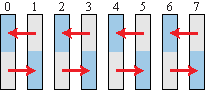
\includegraphics[scale=.75]{binary-swap-1}
\end{wrapfigure}
Binary swap occurs on a series of iterations.
In the first iteration, processes group in adjacent pairs.
The processes exchange halves of their image, as shown at right.

\begin{wrapfigure}{r}{0pt}
  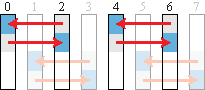
\includegraphics[scale=.75]{binary-swap-2}
\end{wrapfigure}
For the next iteration, all the process subdivide into the group of processes holding the same image, and then repeat the process.
In the example at right with 8 processes, highlighted processes 0, 2, 4, and 6 group together and split their remaining images.
(The remaining processes form their own group and similarly subdivide.)

\begin{wrapfigure}{r}{0pt}
  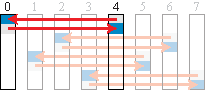
\includegraphics[scale=.75]{binary-swap-3}
\end{wrapfigure}
Binary swap iterations continue until each process has a unique portion of the image.
In our example with 8 processes, binary swap completes after the third iteration.
In general, binary swap takes $\log_{2}p$ iterations, where $p$ is the number of processes.

\subsection{Binary Swap Variations for Odd Process Factors}
\label{sec:BinarySwapVariations}

Binary swap has many desirable qualities.
The number of iterations grows slowly with respect to the number of processes.
Also, each iteration halves the amount of work required per process.
In total, each process will send, receive, and process no more than the number of pixels in a single image.
However, a well known limitation is that binary swap only works when the number of processes is a perfect power of 2.
If there are any odd factors, then at some iteration there will be an odd number of processes in a group and they will not all be able to pair up properly.
In response, there are numerous modifications to binary swap the handle odd factors.

\subsubsection{Naive}

\begin{wrapfigure}{r}{0pt}
  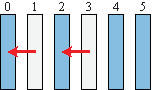
\includegraphics[scale=.75]{naive}
\end{wrapfigure}
The most obvious way to manage odd factors is to find the largest power of 2 less than the number of processes and then offload images from any processes that do not fit in a group that size.
In the example at right, we have 6 processes.
The largest power of 2 less than 6 is 4, so two processes send their images away and drop out of the communication.
The remaining 4 processes do a normal binary swap as outlined in Section \ref{sec:BinarySwap}.

This method has been given multiple names such as \keyterm{reduced}\lcite{23Swap} and \keyterm{folding}\lcite{Moreland2011:SC}.
To avoid confusion from the other techniques (many of which can be thought of as ``reducing'' or ``folding''), this paper refers to this technique as \keyterm{\naive}.

\subsubsection{234 Composite}

One of the big drawbacks of the \naive technique is that it adds another iteration to the compositing.
It also requires the transfer of full images, which potentially doubles the amount of data transferred or computed by each process.
Nonaka \etal\scite{Nonaka2015,Nonaka2018} propose \keyterm{\ttfcomposite} to roll the reduction into the first iteration of the binary swap algorithm.

\Ttfcomposite does this using a combination of \keyterm{3-2 reduction} and \keyterm{4-2 reduction} operations.
These operations take a group of 3 and 4 processes, respectively, and reduce them to a group of 2.
The resulting 2 processes each end with half an image much like a standard binary-swap pair.

\begin{wrapfigure}{r}{0pt}
  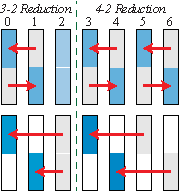
\includegraphics[scale=.75]{234-composite-6-proc}
\end{wrapfigure}
In this example of 7 processes, there is 1 group of of 3-2 reduction and 1 group of 4-2 reduction.
After the operations are complete, there are 4 remaining processes in a state equivalent to have running the first step of binary swap.
The remainder of the algorithm follows that of binary swap.

\subsubsection{Telescoping}

Moreland \etal\scite{Moreland2011:SC} propose the \keyterm{\telescoping} algorithm.
Like the \naive algorithm, \telescoping reduces the problem to groups that are a power of 2.
However, rather than reduce the size of the groups before compositing starts, \telescoping performs this reduction after compositing primarily finishes.
It does this by breaking the processes into a series of groups that are the largest powers of 2 that it can make.
It then runs binary swap on all such groups simultaneously.
When compositing finishes, the smaller groups transfer their images to the larger groups.

\begin{wrapfigure}{3}{0pt}
  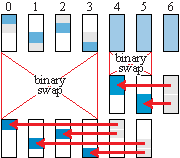
\includegraphics[scale=.75]{telescoping-7-proc}
\end{wrapfigure}
In the example at right, 7 processes are split into a group of 4, a group of 2, and a group of 1 (all perfect powers of 2).
Binary swap is run concurrently and independently on each group.
The group of size 1 splits its image and sends it to the size 2 group.
Subsequently, the size 2 group splits its images and sends them to the size 4 group (thus collapsing the images in a telescoping manner).
Since smaller groups have less work, we can expect the smaller groups to finish more quickly and have its data in transit while the larger groups finish.

%% \begin{wrapfigure}{3}{0pt}
%%   \includegraphics[scale=.75]{telescoping-9-proc}
%% \end{wrapfigure}
%% One odd feature of \telescoping is that small groups might have to send many messages to the next largest group.
%% For example, if compositing with $2^{i} + 1$ processes, the lone process will have to send to $2^{i}$ processes, as demonstrated at right.

\subsubsection{Remainder}

Rather than attempt to reduce the number of processes to a power of 2, another approach is to modify the binary swap algorithm to manage the situation where a group cannot be evenly divided.
A simple approach, which we will refer to as \keyterm{\remainder}, simply rolls the image from any remainder when dividing the processes by employing a single 3-2 reduction to absorb the remainder.
This is roughly equivalent to the reduction technique proposed by Rabenseifner and Tr\"{a}ff\scite{Rabenseifner2004} although, to the author's knowledge, this has not been directly applied to parallel rendering.
(Also, the implementation used in this paper actually uses the overlap variant of 3-2 reduction as proposed by Nonaka\scite{Nonaka2015}.)

\begin{wrapfigure}{3}{0pt}
  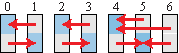
\includegraphics[scale=.75]{remainder-1}
\end{wrapfigure}
In this example of 7 processes to the right, the processes are divided by employing a 3-2 reduction on the last 3 processes.
The last process drops out of the computation at this point.

\begin{wrapfigure}{3}{0pt}
  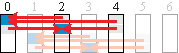
\includegraphics[scale=.75]{remainder-2}
\end{wrapfigure}
The next (and final) iteration has groups of 3.
These again are managed by a 3-2 reduction.
The highlighted processes 0, 2, and 4 blend image data in processes 0 and 2 while dropping process 4.

\subsubsection{2-3 Swap}

All the previous algorithms for odd factors of processes require processes to go idle at some point during the computation.
Yu \etal\scite{23Swap} describe \keyterm{\ttswap}, which can perform image compositing on any number of processes while balancing the computation among all processes at all iterations.
It does so by dividing processes into groups of 2 or 3 and likewise dividing images by 2 and 3.

\begin{wrapfigure}{3}{0pt}
  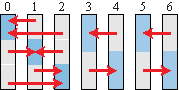
\includegraphics[scale=.75]{2-3-swap-1}
\end{wrapfigure}
For example, in the first step of a 7 process composite, shown at right, splits the processes in a group that does a 3-way swap and 2 more groups that do a 2-way swap.
The details on when \ttswap does a 2-way vs. 3-way swap is complicated and requires precomputing a compositing tree.
For details, see Yu's paper\lcite{23Swap}.

\begin{wrapfigure}{3}{0pt}
  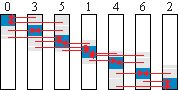
\includegraphics[scale=.75]{2-3-swap-2}
\end{wrapfigure}
After the first step it is notable that the image partitions of processes do not line up as they do for binary swap.
\Ttswap manages this by interlacing the processes that are regrouped and redividing evenly.
(Note the reordering of processes in this example.)
The interlacing ensures that each process receives only pixels that it started with.

\subsection{Alternatives to Binary Swap}
\label{sec:BinarySwapAlternatives}

Finally, we quickly review some alternatives to binary swap that are viable but not considered in this paper.

\keyterm{Direct send}\lcite{DirectSend1} is a simple algorithm that assigns a piece of the image to each process, and then each process sends all its pieces directly to the responsible process.
Direct send minimizes latency because all data reaches its destination in one step, but the number of messages required to do this grows quadratically with respect to the number of processes.
Thus, the technique is unsuitable for large numbers of processes\lcite{Moreland2011:SC}.
An often cited but seldom implemented variant of direct send is \keyterm{Scheduled Linear Image Compositing} (SLIC)\lcite{SLIC}, which optimizes pixel assignment by assigning non-contiguous image pieces.
%However, SLIC can only be used on regular geometry (to predict what parts of the image are covered), and it is likely to have the same scaling problems as direct send (although this has never been directly studied).

The \keyterm{parallel pipeline} method\lcite{Lee1996} establishes processes in a linear chain where image data is passed down the chain.
Parallel pipeline has a long latency as images must be passed down the entire pipeline, but it has been shown that the regular message passing can be used to optimize for physical hardware connections\lcite{Wu2009}.
\keyterm{Rotate tiling}\lcite{Lin2004} is a variant of parallel pipeline that establishes multiple pipelines to reduce latency.

\keyterm{Radix-k}\lcite{RadixK} combines binary swap and direct send by allowing each iteration of binary swap to group into any size rather than just 2 and uses a direct send in that subgroup to swap data around.
Because it can divide processes in any way, it is not limited to powers of 2 like binary swap.
However, because the performance of radix-k can vary based on factors chosen\lcite{Kendall2010,Moreland2011:SC}, it would be interesting to explore ways to adjust available factors.
However, this is beyond the scope of this paper and left for future work.

\section{Experiments}
\label{sec:Results}

For these experiments, versions of binary swap and the variants described in Section \ref{sec:BinarySwapVariations} were implemented in a common code base.
All the algorithms use a common infrastructure for rendering and image data structures.
This test infrastructure renders a simple scene where each process rendered an opaque box such as shown in Figure \ref{fig:RenderExample}.

\begin{figure}[htb]
  \centering
  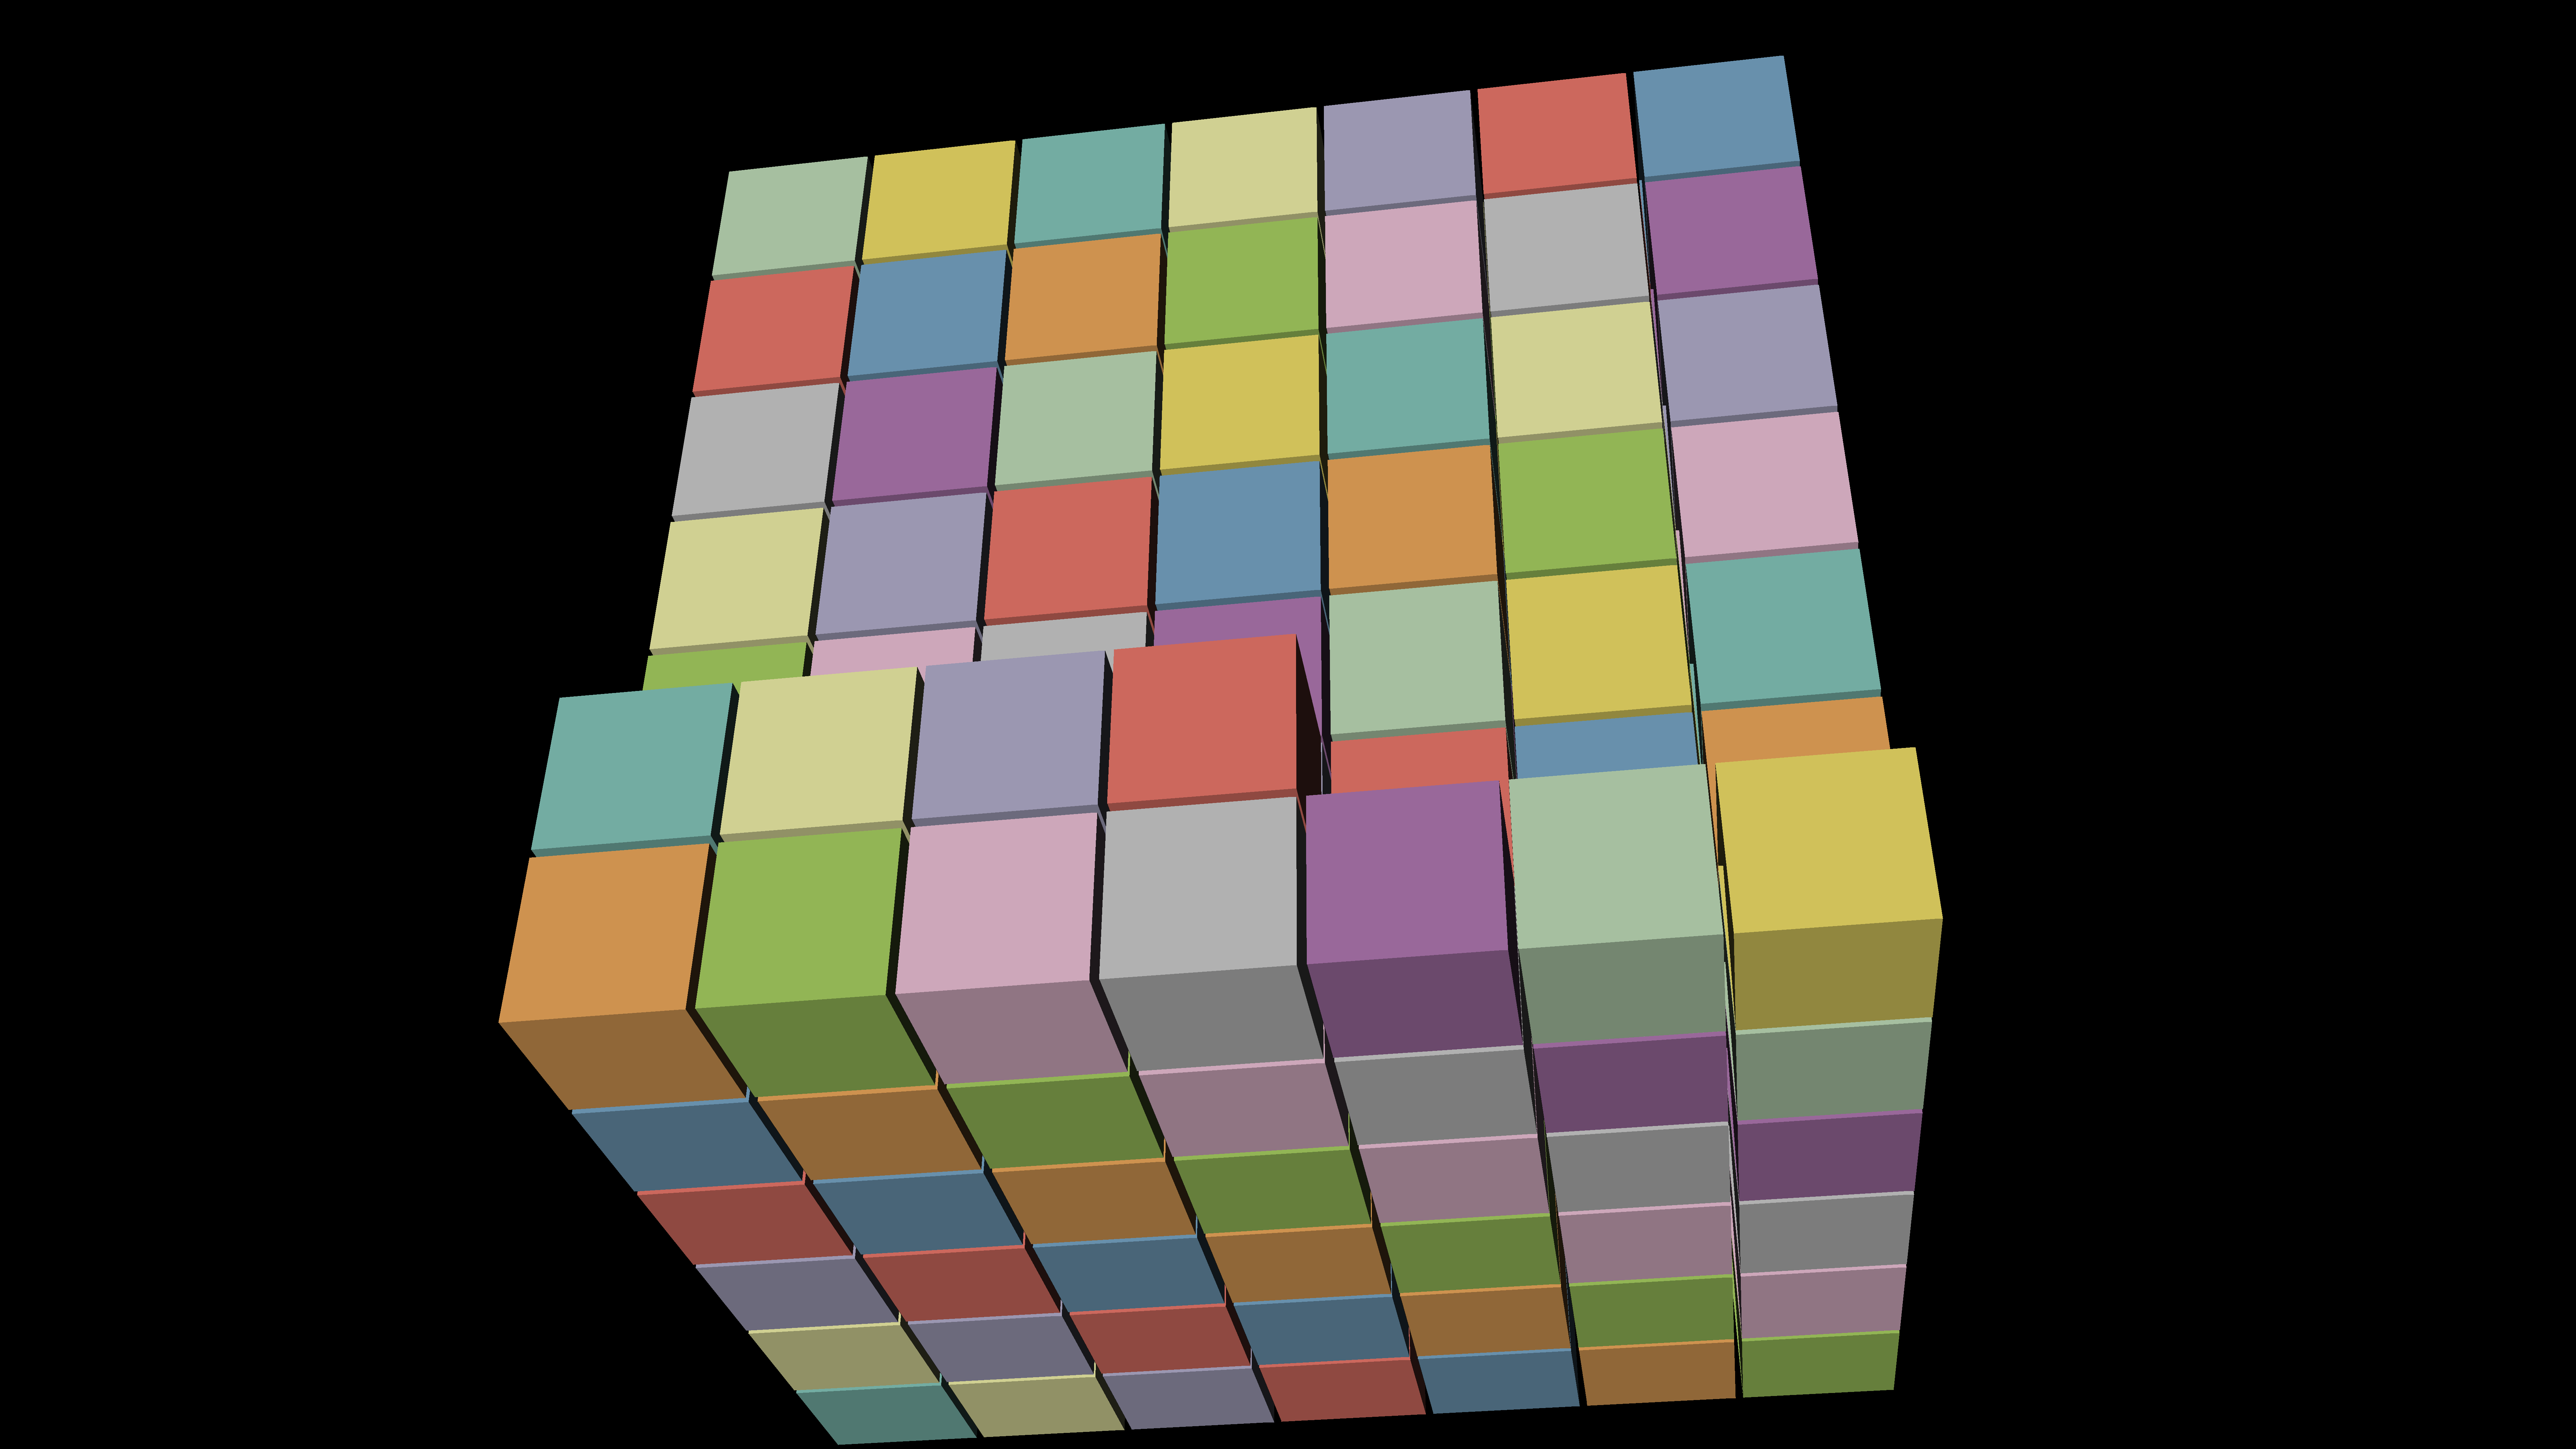
\includegraphics[width=\linewidth]{render-example}
  \caption{An example image rendered during tests.}
  \label{fig:RenderExample}
\end{figure}

The experiments were run on the Sky Bridge cluster at Sandia National Laboratories\lcite{SkyBridge}.
Sky Bridge is a water cooled Cray capacity cluster with 1,848 nodes (although at most 512 nodes were used at any one time during these experiments).
Each node contains 2 2.6 GHz Intel Xeon E5-2670 processors, each with 8 cores (16 cores total).
The nodes are connected with a Infiniband interconnect.
The experiments were run in ``virtual node'' mode where each core ran a separate MPI process (except where specified in Section \ref{sec:VNCompare}).

Each experiment has a minimum of 10 trials (rendered frames).
Each trial is performed from random camera rotations around the geometry (although these random locations are consistent across experiments by using the same pseudorandom number generator seed).
Rendering times for two different image sizes are reported: HDTV ($1920 \times 1080$) and 8K UHD ($7680 \times 4320$).

The compositing engaged active pixel encoding for compression (except where specified in Section \ref{sec:FullImages}).
The times reported here are specifically the time to divide the image and blend pixels.
This leaves the final composited image divided across many MPI processes.
The time to gather the image pieces is not reported except where discussed in Section \ref{sec:Gather}.
The time to map the geometry to pixels is not reported as this time is independent from the compositing algorithm.

\subsection{Algorithm Comparison and Scaling}
\label{sec:Scaling}

The first experiment performs a scaling study of the behavior of the \binaryswap algorithm with the 4 variations discussed in Section \ref{sec:BinarySwapVariations}.
The tests include runs on 64 processes (4 real nodes) up to 8192 cores (512 real nodes).
It is impractical to run an experiment on every possible number of processes.
Instead jobs are chosen such that the number of real nodes where all the prime factors are either 2 or 3.
This hits all jobs sizes that are a perfect power of 2 and many in between at odd spacing.
The results of these experiments are shown in Figures \ref{fig:ScalingHDTV} and \ref{fig:Scaling8K}.
(The plots are labeled as ``Partial Composite Time'' because these times include only splitting the images and blending pixels.
The fully composited image is left in pieces scattered across the MPI processes.
Section \ref{sec:Gather} discusses the collection of these pieces.)

\begin{figure}
  \centering
  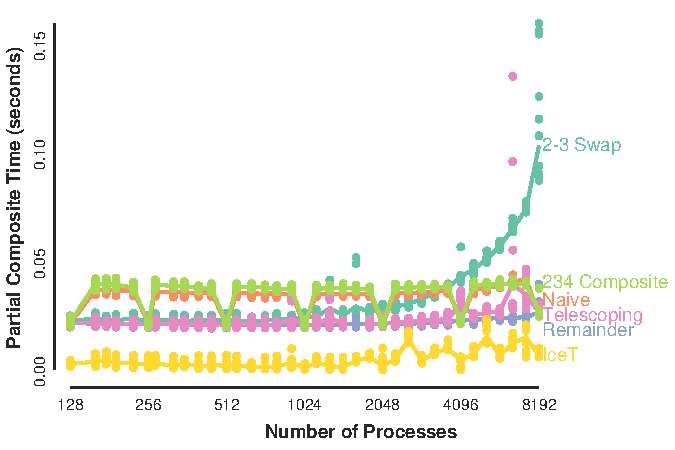
\includegraphics[width=\linewidth]{scaling-hdtv}
  \caption{
    Performance of variations of \binaryswap for HDTV ($1920 \times 1080$) images.
    The performance of the IceT rendering library is also given for reference.
  }
  \label{fig:ScalingHDTV}
\end{figure}

\begin{figure}
  \centering
  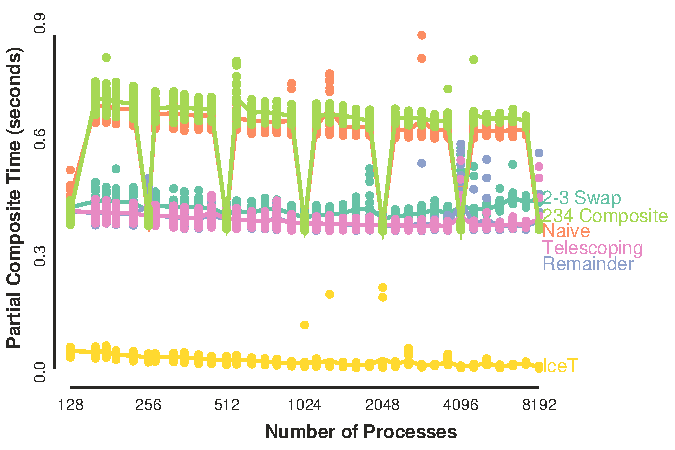
\includegraphics[width=\linewidth]{scaling-8k}
  \caption{
    Performance of variations of \binaryswap for 8K UHD ($7680 \times 4320$) images.
    The performance of the IceT rendering library is also given for reference.
  }
  \label{fig:Scaling8K}
\end{figure}

A first observation about the data is to note that the naive algorithm pays a significant but consistent penalty for running on a number of processes that is not a power of 2.
This is consistent with the findings of Yu et al.\scite{23Swap}.

A second observation is that the \ttswap algorithm behaves well up to 1024 processes (which is as large as was measured by Ye et al.\scite{23Swap}), but the performance starts to deteriorate on larger sizes, particularly for the HDTV images.
This appears to be caused by the time taken to build the compositing tree, which is complex for \ttswap and has to take into account all the processes.
Figure \ref{fig:23SwapOverhead} demonstrates the fraction of time spent in building the 2-3 compositing tree.

\begin{figure}[htb]
  \centering
  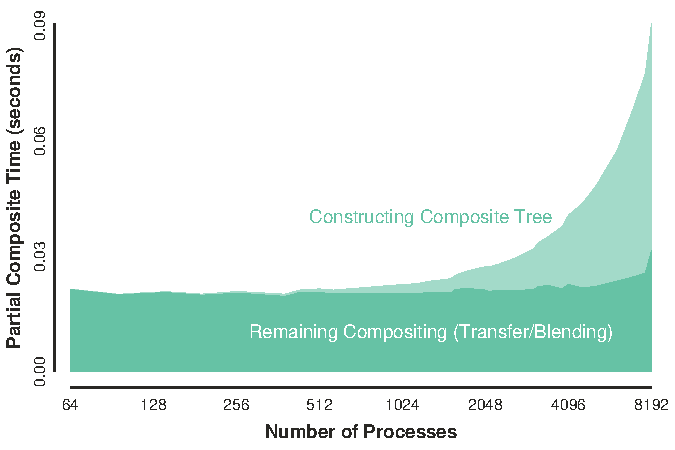
\includegraphics[width=\linewidth]{2-3-swap-overhead}
  \caption{
    Average times for \ttswap compositing.
    The top lighter shade shows the time spent building the compositing tree whereas the bottom darker shade shows the remainder of the algorithm (transferring data, blending colors, etc.).
  }
  \label{fig:23SwapOverhead}
\end{figure}

A third observation is that both the \telescoping and \remainder versions of binary swap perform very well throughout the entirety of the experiments.
This is somewhat counterintuitive for the \remainder algorithm, which, much like the poor performing \naive algorithm, lets processes go idle.
However, unlike the \naive algorithm, \remainder delays letting processes go idle until as late as possible.
More importantly, \remainder has fewer iterations than \naive with each iteration dividing the amount of work done by each process in half.

A fourth observation is that all of the \binaryswap algorithms implemented for our experiment perform less well than the IceT software.
IceT uses a combination of \radixk and \telescoping, but the real performance gain is in its high-speed blending and management of memory to reduce allocation and messages.
In contrast, the experimental code sacrifices some efficiency for readability of code and ease of implementation to facilitate comparisons like those in this paper.

\subsection{No Image Compression}
\label{sec:FullImages}

The compositing reported in Section \ref{sec:Scaling} compresses images during compositing using run lengths of active and inactive pixels (sometimes called \keyterm{active pixel encoding}).
Any practical system should employ active pixel encoding or something like it as previous work has shown dramatic improvements in compositing time\lcite{Ahrens1998,Yang1999,Moreland2001,Takeuchi2003}.
However, active pixel encoding can change the performance behavior of the compositing.
The overall time will increase and decrease depending on the effectiveness of the compression.
Image compression can also add load imbalance.

To verify that active pixel encoding is not artificially skewing the previous results, a second set of runs replicates the experiments with image compression turned off.
This set of experiments only includes the \naive, \ttswap, and \remainder algorithms.
\Telescoping was not run to save time because its performance is similar to \remainder.
IceT was not run because it always compresses the data.
The results are shown in Figures \ref{fig:NoCompressHDTV} and \ref{fig:NoCompress8K}.

\begin{figure}
  \centering
  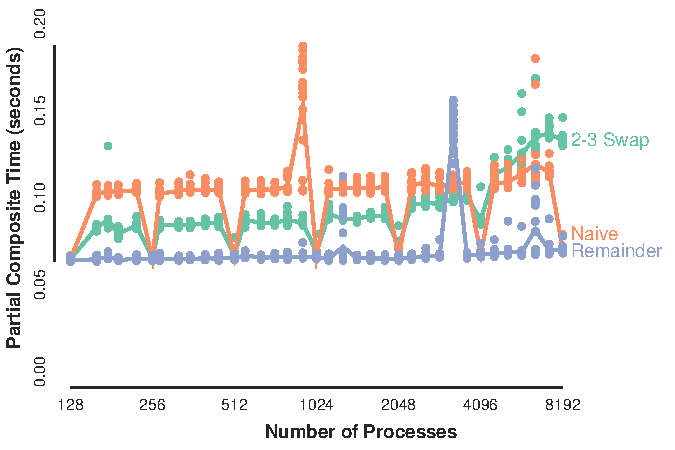
\includegraphics[width=\linewidth]{no-compress-hdtv}
  \caption{
    Performance of compositing algorithms without compression for HDTV ($1920 \times 1080$) images.
  }
  \label{fig:NoCompressHDTV}
\end{figure}

\begin{figure}
  \centering
  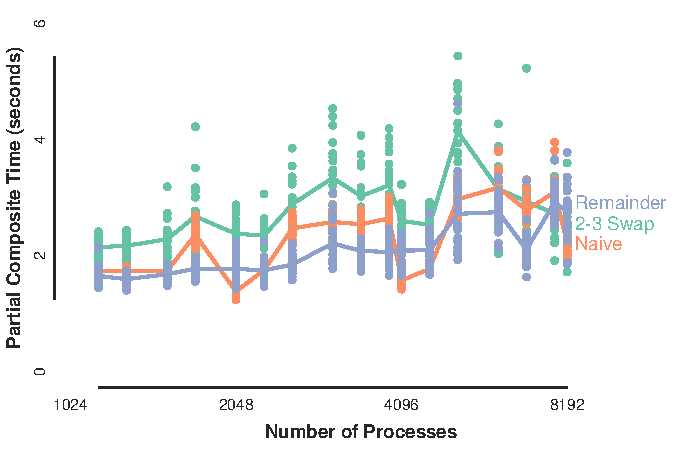
\includegraphics[width=\linewidth]{no-compress-8k}
  \caption{
    Performance of compositing algorithms without compression for 8K UHD ($7680 \times 4320$) images.
  }
  \label{fig:NoCompress8K}
\end{figure}

\begin{figure*}
  \centering
  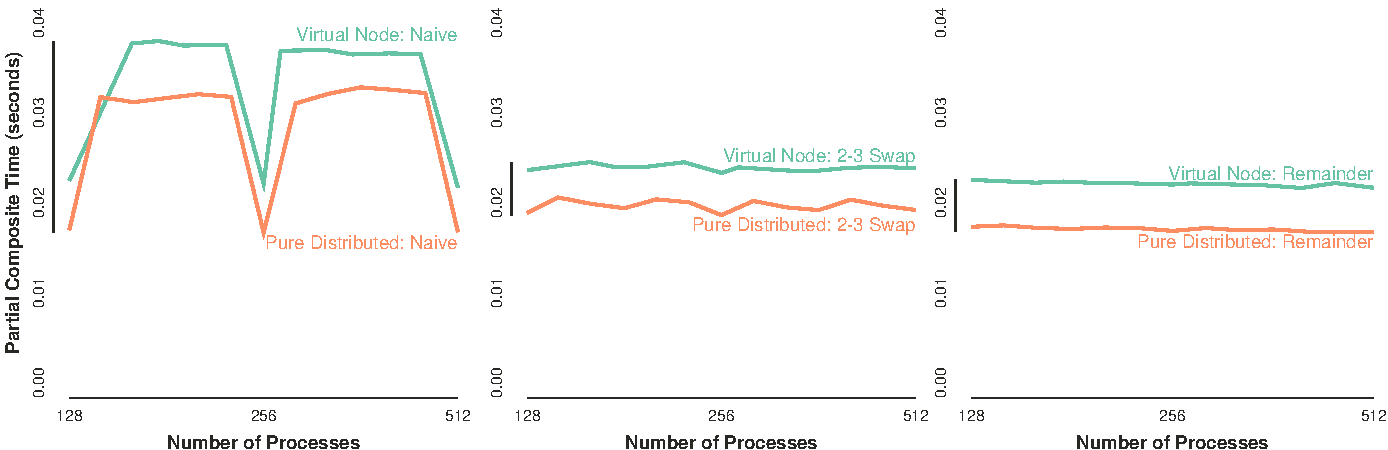
\includegraphics[width=\linewidth]{vn-vs-smp-hdtv}
  \caption{
    A comparison of the performance of compositing when run on the same number of cores in virtual node mode and pure distributed mode when using the \naive, \ttswap, and \remainder algorithms (in the left, center, and right plots, respectively).
  }
  \label{fig:VNvsSMPHDTV}
\end{figure*}

A first observation is that the behavior of the three algorithms is roughly consistent, proportionally speaking, with the behavior using active pixel encoding.
The \naive algorithm pays a large penalty when not using a perfect power of 2 number of processes.
The \ttswap algorithm is insensitive to the factors of the number of processes, but its performance worsens at larger scales.
The \remainder algorithm's performance is consistent and is one of the best performers in all cases.

A second observation is that without compression, the compositing takes about 3.5 to 4.5 times as long, which verifies the statements about the utility of active pixel encoding during compositing.

A third observation is that the variance of the run time, both from trial to trial and the average from job to job, is much larger than that when using active pixel encoding.
This is surprising because removing compression makes the work more consistent and should lead to less variance, not more.
Presumably the time for data communication is not consistent.
Perhaps the extra data on the interconnect are causing contention.

\subsection{Virtual Node vs. Pure Distributed}
\label{sec:VNCompare}

To maximize the scaling in the aforementioned experiments, runs were performed in a \keyterm{virtual node} mode where each core on a node has its own MPI process.
In essence, each core is treated as a separate node even though they technically share resources.
Once consequence of the virtual node setup is that the network behavior is expected to be more heterogeneous.
Data transfers between two virtual nodes on the same physical node are expected to be much faster than transfers between virtual nodes on two different physical nodes.
To ensure that the conclusions we draw are not invalid for different network configurations, the experiments are also run in a \keyterm{pure virtual} mode where only a single MPI process is run on each node (and consequently only one core is used).

Figure \ref{fig:VNvsSMPHDTV} shows the comparison between running on virtual node and pure virtual for generating HDTV images.
A similar run for 8K UHD images was also run and gave similar results, but it is not displayed here for lack of space.

An interesting observation is that the pure distributed mode runs consistently faster than the virtual node mode.
This is counterintuitive as many of the connections in virtual node mode are faster than those in pure distributed mode.
Most likely the slowdown is due to the cores in virtual node mode sharing the same network interface controller (NIC) and having to divide the bandwidth accordingly.
This measurement suggests that overall rendering throughput will be maximized by leveraging shared-memory local rendering, of which there are many choices\lcite{OpenSWR,Wald2014,Knoll2014,Larsen2015:RayTrace,Moreland2016:VTKm}, to reduce the number of MPI processes on each physical node.

Apart from the consistent overhead of running in virtual node mode, we can see that the characteristics of the behavior are similar for both modes.
Thus, we can conclude that the findings drawn from our virtual node scaling can be applied to other job launching patterns.

\subsection{Aberrant Readings}

For clarity, the results presented in the previous sections have been selected for clarity.
For completeness, this section documents some of the more unusual or inconsistent measurements taken.

\subsubsection{Inconsistent Gather Times}
\label{sec:Gather}

The previously reported compositing times include the process up to the point where the resulting image is divided among multiple processes.
However, in any practical system, the images must be gathered together for display.
It is known that this gathering can take a significant portion of the compositing time\lcite{Rabenseifner2004,Moreland2011:SC,Larsen2016,Nonaka2018}.

The software used for these experiments does this collection with a sequence of MPI\_Gather and MPI\_Gatherv commands.
However, as shown in Figure \ref{fig:GatherTimes}, the cluster used for these experiments is giving wildly different performance for the gather operations that seems to have little to do with the compositing algorithms analized in this paper.

\begin{figure}
  \centering
  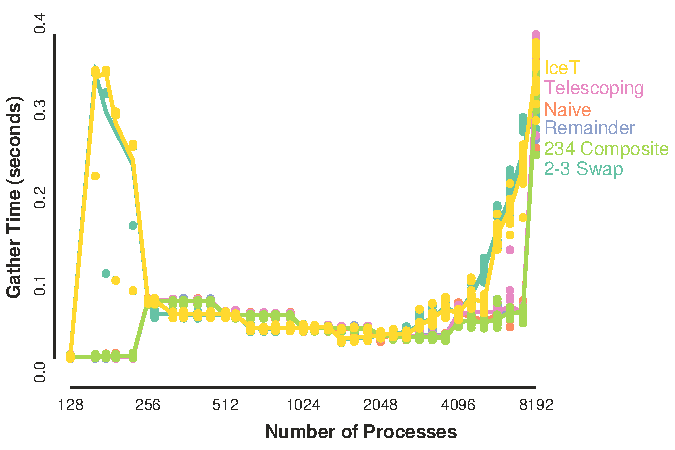
\includegraphics[width=.5\linewidth]{gather-hdtv}%
  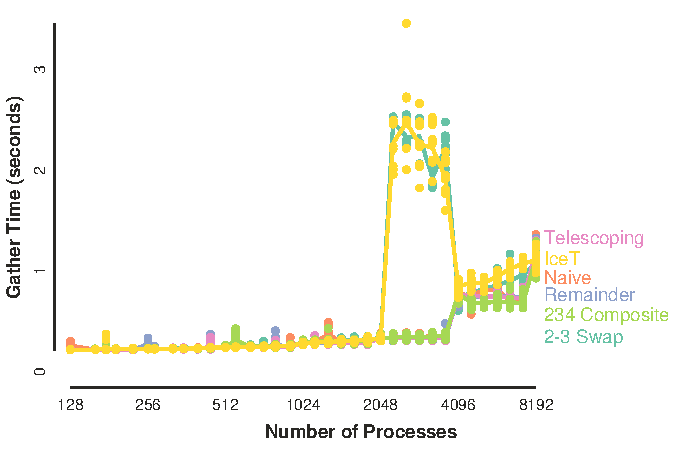
\includegraphics[width=.5\linewidth]{gather-8k}
  \caption{
    The time spent while gathering image data after the partial composite.
    At left are times for HDTV ($1920 \times 1080$) images and at right are times for 8K UHD ($7680 \times 4320$) images.
  }
  \label{fig:GatherTimes}
\end{figure}

These times suggest that a different mechanism for collection is needed.
Nonaka \etal\scite{Nonaka2018} has success by adding padding and process reordering to replace MPI\_Gatherv with MPI\_Gather.
However, in this case it might be better to not rely on MPI-provided collectives at all.

\subsubsection{Errors in 2-3 Swap}
\label{sec:2-3SwapErrors}

Several checks were run during the experiments to ensure the correctness of the compositing algorithms.
For most of the runs there were no problems.
However, during a few of the \ttswap runs bad pixels were detected at the top of the images like those in Figure \ref{fig:BadComposite23Swap}.
It appears to be an indexing problem caused by a race condition that cannot be easily replicated.

\begin{figure}[htb]
  \centering
  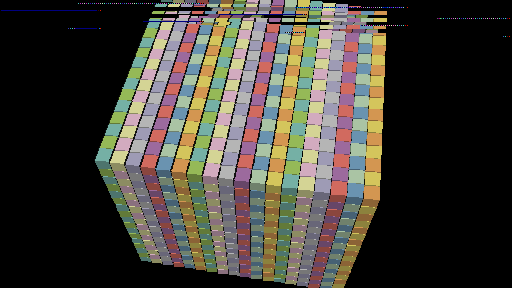
\includegraphics[width=.5\linewidth]{bad-composite-2-3-swap}
  \caption{Compositing errors detected during \ttswap.}
  \label{fig:BadComposite23Swap}
\end{figure}

Although some of the images are incorrect, it seems unlikely that the errors are causing a significant impact in the recorded timings.
Furthermore, since \ttswap is not one of the better performing algorithms, there seems little reason to suffer the aggravation to fix the problem.

\subsubsection{System Slowdowns}

During the experiments it was noticed that some of the runs gave anomalously long run times.
These appear to be intermittent issues with the testing cluster.
Several of these experiments were re-run and found that the extra run time was in fact anomalous.
However, some of the less egregious are left in the results (such as with the spikes seen in Figure \ref{fig:NoCompressHDTV}).

\section{Conclusions}

This paper presents a comprehensive comparative study of many parallel image compositing based on \binaryswap.
Never before have all these algorithms been directly compared, and the results buck some previously accepted notions.

The clear and surprise winner of the comparison is the \remainder version of binary swap.
\Remainder is simple to implement (the implementation used in these experiments has less lines of code than even the \naive algorithm) and is consistently a top performer.
In contrast, \ttfcomposite's is over twice as long as \remainder's (according to cloc\lcite{cloc}) but seldom performs better than \naive.
The implementation for \ttswap is almost 4 times as long as \remainder, and, in the authors subjective experience, much more difficult to implement.

Also surprisingly, the simple but effective \remainder technique does not seem to be used at all in previous literature of parallel rendering.
Ultimately, the parallel rendering research community should stop attempting to find complex solutions to manage undesirable factors but rather use a simple technique to absorb the remaining images when using factors that do not divide processes evenly.

%% if specified like this the section will be committed in review mode
\acknowledgments{
  This material is based upon work supported by the U.S.
  Department of Energy, Office of Science, Office of Advanced Scientific Computing Research, under Award Number 14-017566.

  This paper describes objective technical results and analysis.
  Any subjective views or opinions that might be expressed in the paper do not necessarily represent the views of the U.S.
  Department of Energy or the United States Government.
  Sandia National Laboratories is a multimission laboratory managed and operated by National Technology \& Engineering Solutions of Sandia, LLC, a wholly owned subsidiary of Honeywell International Inc., for the U.S.
  Department of Energy's National Nuclear Security Administration under contract DE-NA0003525.
}

%\bibliographystyle{abbrv}
%\bibliographystyle{abbrv-doi}
\bibliographystyle{abbrv-doi-narrow}
%\bibliographystyle{abbrv-doi-hyperref}
%\bibliographystyle{abbrv-doi-hyperref-narrow}

\bibliography{BinarySwapNon2}
\end{document}
